% \documentclass[12pt,compress,english,utf8,t,usenames,dvipsnames]{beamer}
\documentclass[12pt,compress,english,utf8,t,usenames,dvipsnames,handout]{beamer}
\usepackage[ngerman, english,main=english]{babel}


\title{Hierarchical Temporal Memory}
\subtitle{Biological And Machine Intelligence}
\author{Felix Karg}


\graphicspath{ {../template/} {./graphics/} {../template_tex/} } % add further graphics paths here



\usepackage{etex}
\usepackage{graphicx}
\usepackage[export]{adjustbox}
\usepackage{multicol}
\usepackage{pdfpcnotes}
\usepackage{pdfpages}
% \usepackage[dvipsnames]{xcolor}


% \usepackage{minted}
% \usemintedstyle{pastie}


\usetheme[numbering=fraction, progressbar=frametitle]{metropolis}


\date{December 29, 2020}
% \date{12. Juli 2019}


% \institute{Add Your Institute here}
% \titlegraphic{\vspace{4cm} \hspace{7cm} \includegraphics[height=2cm]{Logo_INST}}
% \titlegraphic{\vspace{4cm} \hspace{7cm} \Huge\LaTeX}

\iftwocols
\AtBeginSection[]
{
    \large
    \begin{frame}{Agenda}
        \begin{multicols}{2}
            \tableofcontents[currentsection]
        \end{multicols}
        \clearpage
    \end{frame}
}

\AtBeginSubsection[]
{
    \large
    \begin{frame}{Agenda}
        \begin{multicols}{2}
            \tableofcontents[currentsection,currentsubsection]
        \end{multicols}
        \clearpage
    \end{frame}
}

\else

\AtBeginSection[]
{
    \large
    \begin{frame}{Agenda}
        \tableofcontents[currentsection]
        \clearpage
    \end{frame}
}

\AtBeginSubsection[]
{
    \large
    \begin{frame}{Agenda}
        \tableofcontents[currentsection,currentsubsection]
        \clearpage
    \end{frame}
}
\fi


\begin{document}

\maketitle

% multicols from:
% https://tex.stackexchange.com/questions/24343/splitting-toc-into-two-columns-on-single-frame-in-beamer

%%%%%%%%%%%%%%%%%%%%%%%%%%%%%%%%%%%%%%%%%%%%%%%%%%%%%%%%%%%%%%%%%%%%%%%%%%%%%%%%%%%%%%%%%%%%%%%%%%%%%%%%%%%%%%%%%%%

\iftwocols
\begin{frame}{Agenda}
    \large
    \begin{multicols}{2}
%        \tableofcontents[hidesubsections]
        \tableofcontents[]
    \end{multicols}
    % \clearpage
\end{frame}

\else

\begin{frame}{Agenda}
    \large
%   \tableofcontents[hidesubsections]
    \tableofcontents[]
    % \clearpage
\end{frame}
\fi


\newcommand{\code}[1]{
    \begin{center}
    \setlength{\fboxrule}{1pt}
    \setlength{\fboxsep}{8pt}
        {\fbox{\parbox{0.81\textwidth}{#1}}}
   \end{center}
}

\newenvironment{codeboxed}[1]
        {\begin{minipage}{\linewidth}\begin{center}#1\\[1ex]\begin{tabular}{|p{\textwidth}|}\hline}
        {\\\hline\end{tabular}\end{center}\end{minipage}}


\newcommand{\backupbegin}{
   \newcounter{finalframe}
   \setcounter{finalframe}{\value{framenumber}}
}

\newcommand{\backupend}{
   \setcounter{framenumber}{\value{finalframe}}
}


\newcommand{\mailto}[1]{
    \href{mailto:#1}{#1}
}

\newcommand{\todo}[1]{
    {\Large\color{red}{(TODO: #1)}}
}

% \definecolor{green1}{RGB}{38, 69, 37} % #264525
\definecolor{green1}{RGB}{72, 129, 69} % #488145
% \definecolor{blue1}{RGB}{7, 43, 94} % #072b5e
\definecolor{blue1}{RGB}{14, 82, 179} % #0e52b3
% \definecolor{violet1}{RGB}{58, 38, 68} % #3a2644
\definecolor{violet1}{RGB}{108, 72, 126} % #6c487e
% \definecolor{orang1}{RGB}{, , 0} % #663400
\definecolor{orang1}{RGB}{193, 98, 0} % #c16200


\newcommand{\green}[1]{
    \textcolor{green1}{#1}
}
\newcommand{\blue}[1]{
    \textcolor{blue1}{#1}
}
\newcommand{\vio}[1]{
    \textcolor{violet1}{#1}
}
\newcommand{\orang}[1]{
    \textcolor{orang1}{#1}
}

% 
\usepackage{etex}
\usepackage{graphicx}
\usepackage[export]{adjustbox}
\usepackage{multicol}
\usepackage{pdfpcnotes}
\usepackage{pdfpages}
% \usepackage[dvipsnames]{xcolor}


% \usepackage{minted}
% \usemintedstyle{pastie}


\usetheme[numbering=fraction, progressbar=frametitle]{metropolis}


\date{December 29, 2020}
% \date{12. Juli 2019}


% \institute{Add Your Institute here}
% \titlegraphic{\vspace{4cm} \hspace{7cm} \includegraphics[height=2cm]{Logo_INST}}
% \titlegraphic{\vspace{4cm} \hspace{7cm} \Huge\LaTeX}

\iftwocols
\AtBeginSection[]
{
    \large
    \begin{frame}{Agenda}
        \begin{multicols}{2}
            \tableofcontents[currentsection]
        \end{multicols}
        \clearpage
    \end{frame}
}

\AtBeginSubsection[]
{
    \large
    \begin{frame}{Agenda}
        \begin{multicols}{2}
            \tableofcontents[currentsection,currentsubsection]
        \end{multicols}
        \clearpage
    \end{frame}
}

\else

\AtBeginSection[]
{
    \large
    \begin{frame}{Agenda}
        \tableofcontents[currentsection]
        \clearpage
    \end{frame}
}

\AtBeginSubsection[]
{
    \large
    \begin{frame}{Agenda}
        \tableofcontents[currentsection,currentsubsection]
        \clearpage
    \end{frame}
}
\fi


\begin{document}

\maketitle

% multicols from:
% https://tex.stackexchange.com/questions/24343/splitting-toc-into-two-columns-on-single-frame-in-beamer

%%%%%%%%%%%%%%%%%%%%%%%%%%%%%%%%%%%%%%%%%%%%%%%%%%%%%%%%%%%%%%%%%%%%%%%%%%%%%%%%%%%%%%%%%%%%%%%%%%%%%%%%%%%%%%%%%%%

\iftwocols
\begin{frame}{Agenda}
    \large
    \begin{multicols}{2}
%        \tableofcontents[hidesubsections]
        \tableofcontents[]
    \end{multicols}
    % \clearpage
\end{frame}

\else

\begin{frame}{Agenda}
    \large
%   \tableofcontents[hidesubsections]
    \tableofcontents[]
    % \clearpage
\end{frame}
\fi


\newcommand{\code}[1]{
    \begin{center}
    \setlength{\fboxrule}{1pt}
    \setlength{\fboxsep}{8pt}
        {\fbox{\parbox{0.81\textwidth}{#1}}}
   \end{center}
}

\newenvironment{codeboxed}[1]
        {\begin{minipage}{\linewidth}\begin{center}#1\\[1ex]\begin{tabular}{|p{\textwidth}|}\hline}
        {\\\hline\end{tabular}\end{center}\end{minipage}}


\newcommand{\backupbegin}{
   \newcounter{finalframe}
   \setcounter{finalframe}{\value{framenumber}}
}

\newcommand{\backupend}{
   \setcounter{framenumber}{\value{finalframe}}
}


\newcommand{\mailto}[1]{
    \href{mailto:#1}{#1}
}

\newcommand{\todo}[1]{
    {\Large\color{red}{(TODO: #1)}}
}

% \definecolor{green1}{RGB}{38, 69, 37} % #264525
\definecolor{green1}{RGB}{72, 129, 69} % #488145
% \definecolor{blue1}{RGB}{7, 43, 94} % #072b5e
\definecolor{blue1}{RGB}{14, 82, 179} % #0e52b3
% \definecolor{violet1}{RGB}{58, 38, 68} % #3a2644
\definecolor{violet1}{RGB}{108, 72, 126} % #6c487e
% \definecolor{orang1}{RGB}{, , 0} % #663400
\definecolor{orang1}{RGB}{193, 98, 0} % #c16200


\newcommand{\green}[1]{
    \textcolor{green1}{#1}
}
\newcommand{\blue}[1]{
    \textcolor{blue1}{#1}
}
\newcommand{\vio}[1]{
    \textcolor{violet1}{#1}
}
\newcommand{\orang}[1]{
    \textcolor{orang1}{#1}
}




\newif\ifonline
\onlinefalse
% \onlinefalse


%%%%%%%%%%%%%%%%%%%%%%%%%%%%%%%%%%%%%%%%%%%%%%%%%%BEGINNING%%%%%%%%%%%%%%%%%%%%%%%%%%%%%%%%%%%%%%%%
% % \section{Examples}

\begin{frame}[c]
     Here a citation: \cite{benchcpp}
\end{frame}

\begin{frame}[c]{Example slide}
    \Large
    \begin{itemize}[<+->]
        \item First Element
        \item Second Element
        \item Third Element
    \end{itemize}
\end{frame}

\begin{frame}[c]{Other example slide}
    \Large
    \begin{itemize}[<+(1)->]
        \item First Element
        \item Second Element
        \item Third Element
    \end{itemize}
\end{frame}

\begin{frame}[c]{Yet another example slide}
    \Large
    \begin{itemize}
        \item First Element
            \pause
        \item Second Element
            \pause
        \item Third Element
    \end{itemize}
\end{frame}








\section{What is Intelligence?}


\begin{frame}[c]{Tests for Intelligence}
    \Large
    \begin{itemize}[<+(1)->]
        \item Turing test
        \item 'IQ' tests
        \item Problme solving tests
        \item Tests for behaviour
        \item ...
    \end{itemize}
\end{frame}


\begin{frame}[c]{Defining Intelligence}
    \pause
    \Huge
    What does the brain \textbf{do} \newline all the time?

    \vfill

    \phantom{Predict. Learn.}
\end{frame}



\section{Biology Recap}

% \begin{frame}[c]{The Human Brain in Numbers}
%     \normalsize
%     \begin{tabular}{ll}
%         & \textbf{Human brain} \\
%         \hline
%         Brain mass & 1508g \\
%         Total number of neurons in brain & 86 billion \\
%         Total number of non-neurons in brain & 85 billion \\
%         Mass, celebral cortex & 1233g \\
%         Neurons, celebral cortex & 16 billion \\
%         Rel. size of the cerebral cortex & 82\% of brain mass \\
%         Rel. n. of neurons in cerebral cortex & 19\% of brain neurons \\
%         Rel. n. of neurons in cerebellum & 80\% of brain neurons \\
%         Mass, cerebellum & 154g \\
%         Neurons, cerebellum & 69 billion \\
%         Rel. size of the cerebellum & 10\% of brain mass\\
%         \hline
%     \end{tabular}
%     \newline
%     \newline
%     Data from \cite{herculano2009human}.
% \end{frame}


\begin{frame}[c]{The Human Brain in Numbers}
    \pause
    \begin{tabular}{ll}
        % & \textbf{Human brain} \\ \\
        Neurons in brain (total) & 86 billion (100\%) \\ \hline \pause
        Neurons in cerebellum & 69 billion (80\%) \\ \pause
        % Rel. neurons in cerebellum & 80\% of brain neurons \\ \pause
        Rel. size of cerebellum & 10\% of brain \\ \hline \pause
        Neurons in celebral cortex & 16 billion (19\%) \\ \pause
        % Rel. neurons in cerebral cortex & 19\% of brain neurons \\ \pause
        Rel. size of cerebral cortex & 82\% of brain \\ \hline \pause
        Neurons in brain stem & 1 billion (1\%) \\
    \end{tabular}
    \newline
    \newline
    \newline
    Data from \cite{herculano2009human}.
\end{frame}


\begin{frame}[c]{The Human Brain}
    \includegraphics[width=0.9\textwidth]{Brain_Side} \\
    \normalsize
    Image from \cite{figsidebrain}.
\end{frame}


\begin{frame}[c]{The Human Brain - Different Areas}
    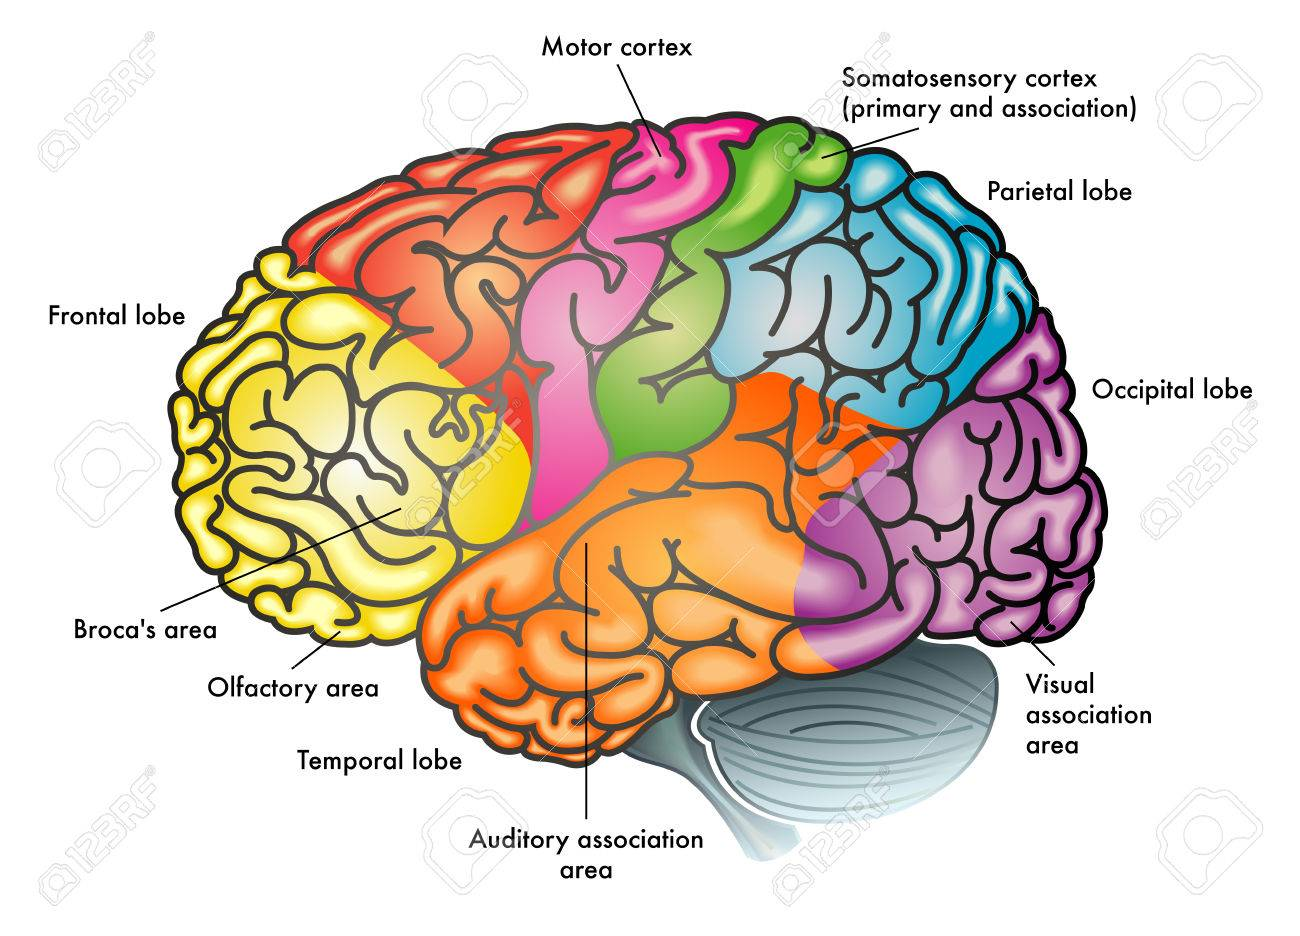
\includegraphics[width=0.9\textwidth]{areas_brain} \\
    \normalsize
    Roberto Biasini © 123RF.com
\end{frame}


\begin{frame}[c]{Cortical Column}
    \Large
    ``There is nothing visual about the visual cortex, and nothing auditory about the auditory cortex``
    \newline
    \phantom{AA} - Vernon Mountcastle
\end{frame}

\begin{frame}[c]{Cortical Column}
    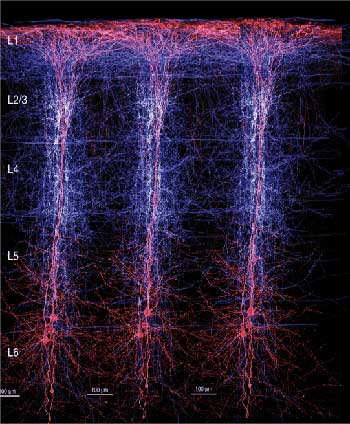
\includegraphics[height=0.95\textheight]{cortical_column}
    \normalsize
    Image from \cite{figcorticalcolumn}.
\end{frame}


\begin{frame}[c]{Cortical Column}
    \Large
    \begin{itemize}[<+->]
        \item Everywhere in the Brain
        \item 80-120 up to 200-400 Neurons
        \item Smallest symbol unit
        \item Activity has meaning
    \end{itemize}
\end{frame}


% \begin{frame}[c]{Cortical Column}
%     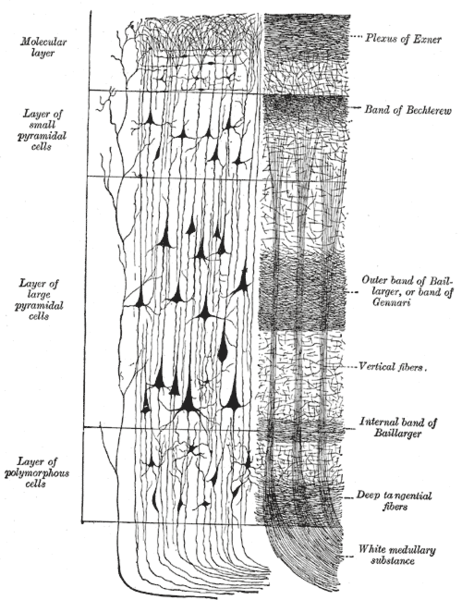
\includegraphics[height=0.95\textheight]{column_2}
%     \normalsize
%     Image from \cite{figcolum2}
% \end{frame}

\begin{frame}[c]{Neuron - Number of Connections}
    \pause
    \vfill % some empty space here
    \begin{tabular}{ll}
        Min. n. of connections \phantom{AAA} & 1'000 \\
        Avg. n. of connections & 7'000 \\
        Max. n. of connections & 10'000 \\ \\ \pause
        % Min. Firing rate & 1 Hz \\
        Firing Rate & 20-250 Hz (453 Hz \cite{wang2016firing}) \\
    \end{tabular}
    \newline
    \vfill
    \small
    Connection data from \cite{herculano2009human} and firing rate from \cite{impact2015firing}.
\end{frame}


\begin{frame}[c]{Neuron - Spike Frequencies}
                                        % trim = left bottom right top
    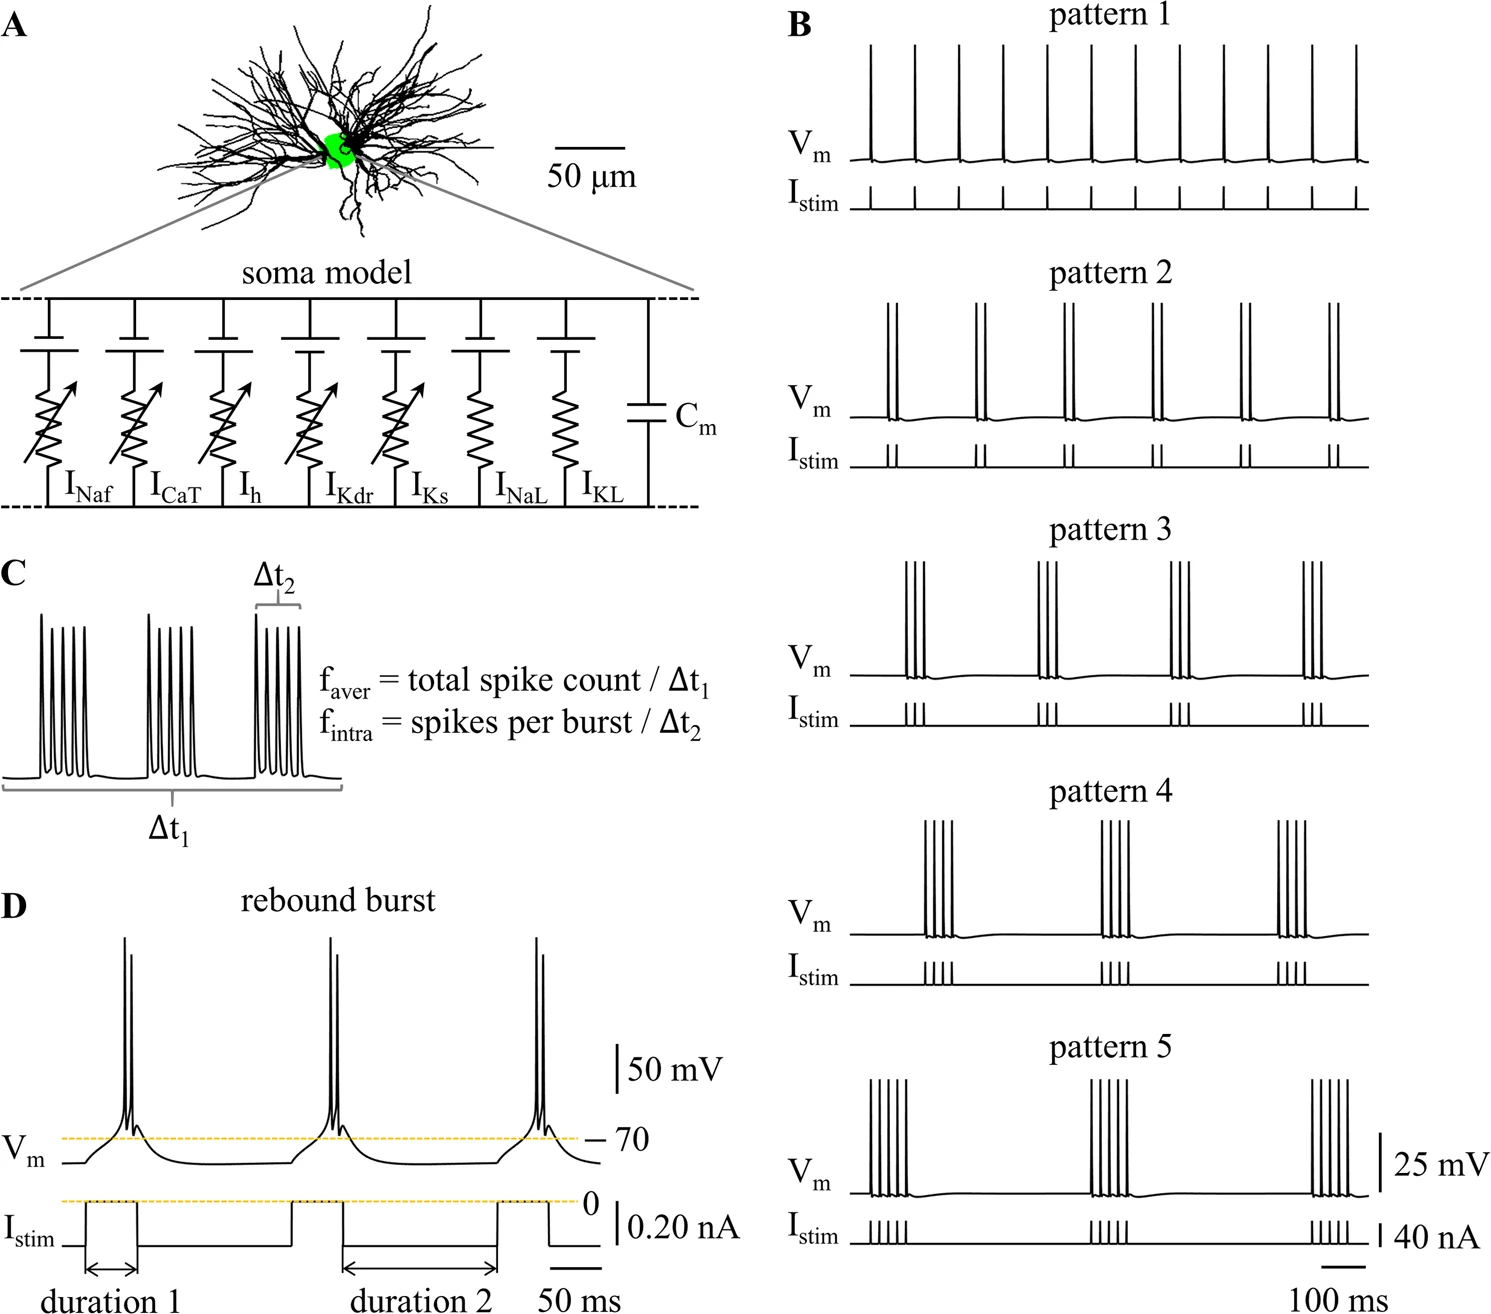
\includegraphics[width=\textwidth, trim=0 460 750 550,clip]{spike_frequency} \\
    \normalsize
    Image adapted from \cite{yi2019average}.
\end{frame}


\begin{frame}[c]{Neuron - Overview}
    % put here: picture of neuron, focus: axons vs dendrites
    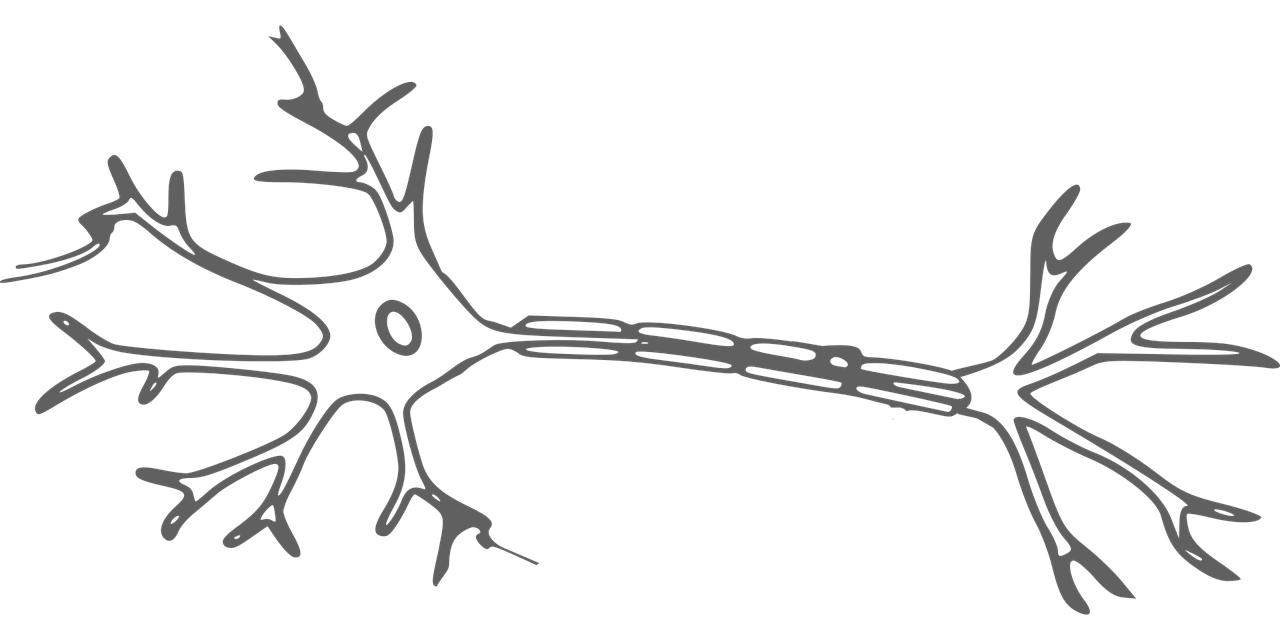
\includegraphics[width=\textwidth]{neuron} \\
    Image from \cite{figneuron}.
    % Image by <a href="https://pixabay.com/users/OpenClipart-Vectors-30363/?utm_source=link-attribution&amp;utm_medium=referral&amp;utm_campaign=image&amp;utm_content=2022398">OpenClipart-Vectors</a> from <a href="https://pixabay.com/?utm_source=link-attribution&amp;utm_medium=referral&amp;utm_campaign=image&amp;utm_content=2022398">Pixabay</a>
\end{frame}


\section{Overview}


\begin{frame}[c]{What is HTM?}
    \begin{itemize}[<+(1)->]
        \item biologically constrained \textbf{theory of intelligence}
        \item originally described in ''On Intelligence''
        \item \textbf{based on neuroscience} of the brain
    \end{itemize}

    \vspace{0.5cm}

    \pause

    $\rightarrow$ Learning Algorithms \pause (of the brain)
\end{frame}


\begin{frame}[c]{Attributes of HTM Algorithms}
    \begin{itemize}[<+(1)->]
        \item can store, learn, infer and recall higher-order sequences
        \item learns unsupervised time-based patterns in unlabeled data on continuous streams
        \item robust against noise
        \item can learn multiple patterns at once
        \item suited for prediction, anomaly detection, classification
        \item tested and implemented in software
        \item commercially used
    \end{itemize}
\end{frame}





\section{Core Concepts}

\subsection{Hierarchy}


\begin{frame}[c]{Why Hierarchy?}
    \Large
    \pause
    If there is a connection cost, hierarchies are more efficient \cite{mengistu2016evolutionary}. 
    
    \pause
    Especially when tasks change regularly.
\end{frame}


\begin{frame}[c]{Why Hierarchy? II}
    \Large
    \begin{itemize}[<+(1)->]
        \item Reduced Training Time
        \item Reduced Memory Usage
        \item Introduce Generalizations
        \item Learned patterns are recombined at higher levels
        \item Transfer Learning
    \end{itemize}
\end{frame}


\begin{frame}[c]{What Hierarchy}
    \pause
                                        % trim = left bottom right top
    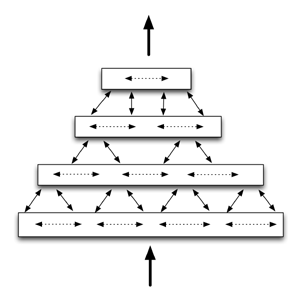
\includegraphics[width=\textwidth, trim = 0 55 0 60, clip]{hierarchy}
\end{frame}


\begin{frame}[c]{Example Application}
    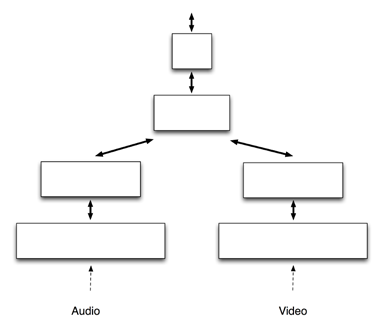
\includegraphics[height=0.9\textheight]{hierarchy_2} 
\end{frame}


\begin{frame}[c]{How Many Levels?}
    \Large
    \begin{itemize}[<+(1)->]
        \item They always learn the best representation
        \item Tradeoff between depth and layer size
        \item Simple problems can be solved with one region
    \end{itemize}
\end{frame}



\subsection{Regions}


\begin{frame}[c]{Region - Introduction}
    \pause
                                        % trim = left bottom right top
    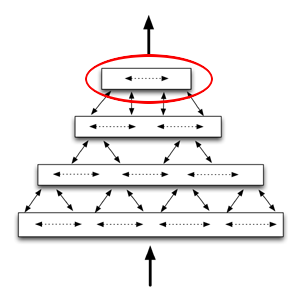
\includegraphics[width=\textwidth, trim = 0 55 0 54, clip]{region}
\end{frame}


\begin{frame}[c]{Region - Details}
    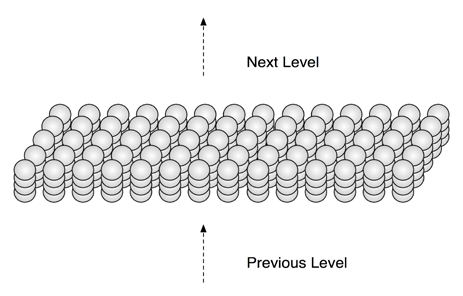
\includegraphics[width=\textwidth]{region_2}
\end{frame}


\begin{frame}[c]{Region - Attributes}
    \begin{itemize}[<+(1)->]
        \item All Regions do basically the same
        \item Based on Biological Regions in the Brain
        \item HTM Regions are similar to Layer 3 of the Neocortex
        \item Can do Inference and Prediction even on complex data
    \end{itemize}
\end{frame}




\subsection{Sparse Distributed Representation}
% \subsection{The Datastructure of the Brain}


\begin{frame}[c,fragile]{Data Saving - Computer Science Solution}
    \Large
    What is \verb|01100101|? \pause Could be either one of:
    % What is ? Could be:
    \begin{itemize}[<+(1)->]
        \item Booleans (\verb|False, True, True, False,|\dots)
        \item Integer (\verb|101|)
        \item Float (\verb|3328.0|)
        \item (Byte-) String (\verb|'e'|)
        \item Pointer to something else
        \item Part of some other Datastructure
    \end{itemize}
\end{frame}


\begin{frame}[c,standout]
    Biological observation: \newline
    We use only part of our brain!
\end{frame}


\begin{frame}[c]{Sparse Distributed Representation - Introduction}
    \Large
    \begin{itemize}[<+(1)->]
        \item Datastructure of the brain
        \item Sparse (around 2\% are active)
        \item Distributed (clusters are somewhat rare)
        \item Inhibitory mechanisms
        \item Neuron states actually have 'meaning'
        \item Combined, they give context as well
        \item Many mechanisms in the brain would not work otherwise
    \end{itemize}
\end{frame}


\begin{frame}[c]{Sparse Distributed Representation - Example}
    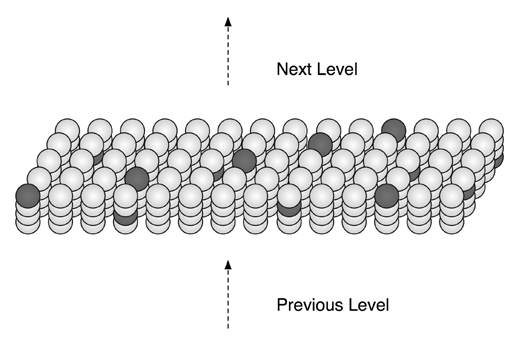
\includegraphics[width=0.95\textwidth]{region_sparse}
\end{frame}


\begin{frame}[c]{Sparse Distributed Representation - Example}
    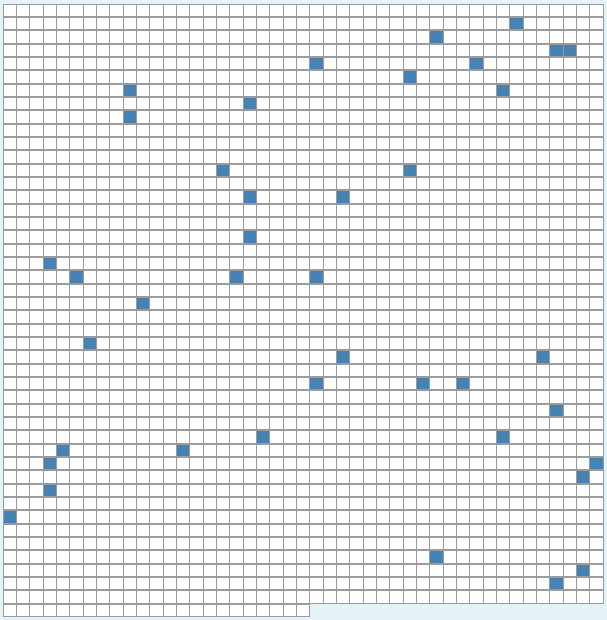
\includegraphics[height=0.9\textheight]{sdr_example}
\end{frame}

% \begin{frame}[c]
    % 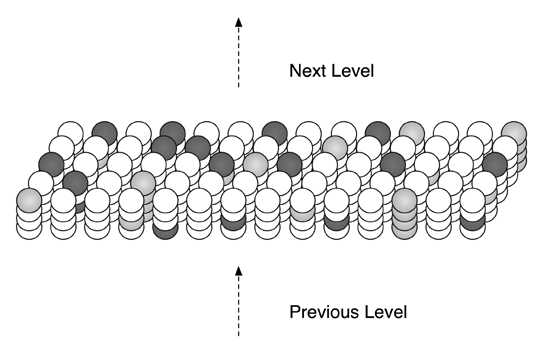
\includegraphics[width=0.9\textwidth]{region_predict}
% \end{frame}


\begin{frame}[c,standout]
    Live Demo!
\end{frame}


\begin{frame}[c]{Sparse Distributed Representation - Live Demos}
    \Large
    \begin{itemize}[<+(1)->]
        \item Ep2/Capacity
        \item Ep2/Matching (Noise resistency)
        \item Ep3/Subsampling
        \item Ep4/Classification
        \item Ep4/Union
        \item Ep5/Scalar Encoding
        \item Ep6/Date Encoding
        \item Ep5/RDSE - Number Encoding
    \end{itemize}
\end{frame}


\begin{frame}[c]{Encoders - Conclusion}
    \begin{itemize}[<+(1)->]
        \item Semantically similar data should result in SDRs with overlapping active bits.
        \item The same input should always produce the same SDR as output.
        \item The output should have the same dimensionality (total number of bits) for all inputs.
        \item The output should have similar sparsity for all inputs and have enough one-bits to handle noise and subsampling.
    \end{itemize}

    \normalsize
    \pause
    Cited from \cite{hawkins2016book}.
\end{frame}



\section{Learning}

\subsection{Overview}

\begin{frame}[c]{Learning}
    % \large
    \begin{itemize}[<+(1)->]
        \item Learning is purely statistical
        \item Looking for Spatial and Temporal Patterns
        \item Regions themselves are limited
        \item Automatically adjusts to size of allocated Memory
        \item Automatic On-Line learning
        \item Takes longer to learn high-level concepts with lower levels missing
        \item Only a precursor for inference and prediction
    \end{itemize}
\end{frame}


\begin{frame}[c]{Inference}
    \Large
    \begin{itemize}[<+(1)->]
        \item Matching previously learned sequences
        \item Example: recognizing a melody
        \item There are only novel experiences
        \item Partial SDR matches suffice
    \end{itemize}
\end{frame}


\begin{frame}[c]{Prediction}
    \Large
    \begin{itemize}[<+(1)->]
        \item Matching stored sequences
        \item Can be thought of to be similar to a markov chain
        \item Takes up a considerable amount of memory
        \item Integral to how the brain works
    \end{itemize}
\end{frame}


\begin{frame}[c]{Prediction - Key Properties}
    \Large
    \begin{itemize}[<+(1)->]
        \item Continuity
        \item Occurs everywhere
        \item Context sensitivity
        \item Stability
        \item Anomaly Detection
        \item Noise robustness
    \end{itemize}
\end{frame}





\subsection{Spatial Pooling}


\begin{frame}[c]{Spatial Pooler - Introduction}
    \pause
                                     % trim = left bottom right top
    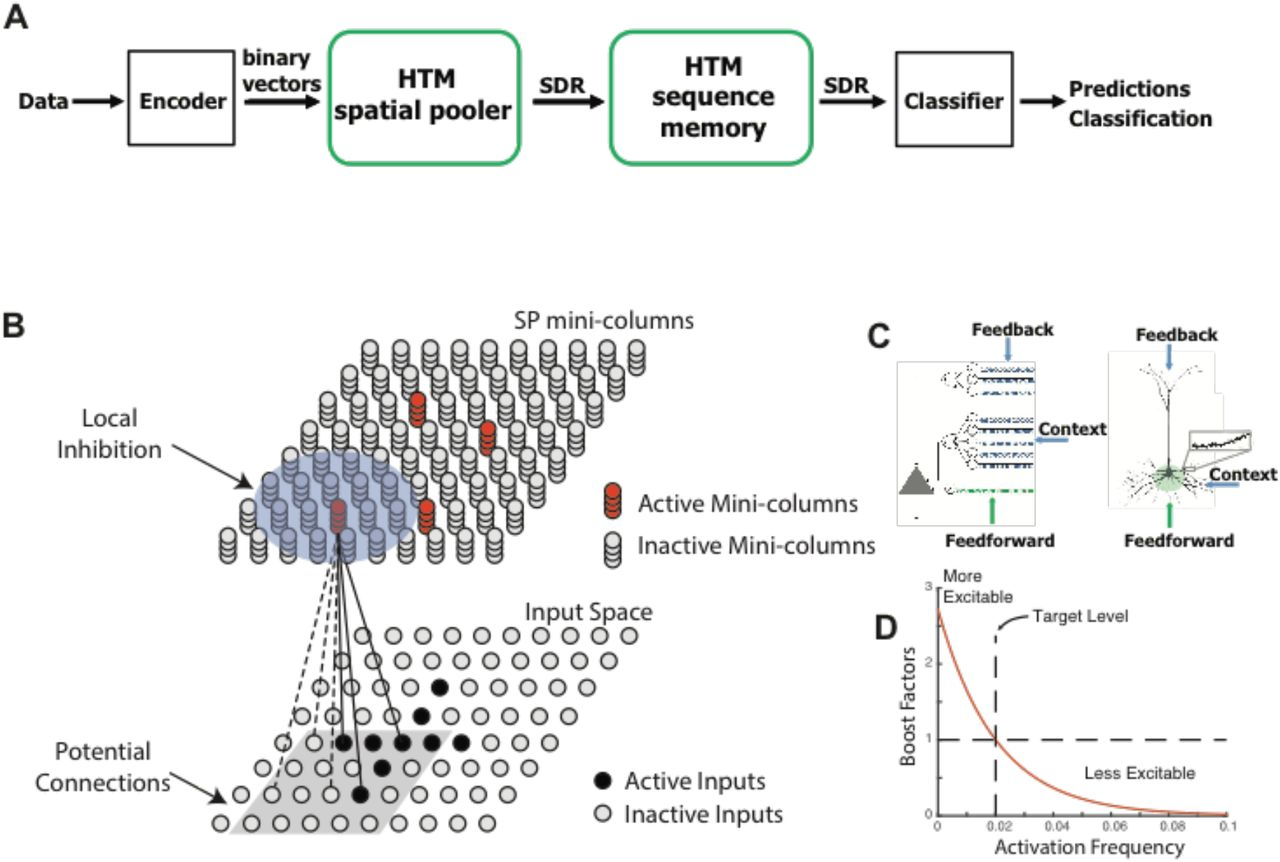
\includegraphics[width=\textwidth, trim= 0 0 97 70, clip]{spatial_pooler} \\
    \normalsize
    Image adapted from \cite{cui2017htm}.
\end{frame}


\begin{frame}[c,fragile]{Spatial Pooler - Connection details}
    \Large
    Show \verb!Ep8/Learning Rules!!
    \newline
    \begin{itemize}[<+(1)->]
        \item Many Connections
        \item Only Columns with highest overlap scores continue
        \item Everyone else gets inhibited
        \item Next: Updating Permanence Values
    \end{itemize}
\end{frame}


\begin{frame}[c,allowframebreaks]{Spatial Pooler - Learning Details}
    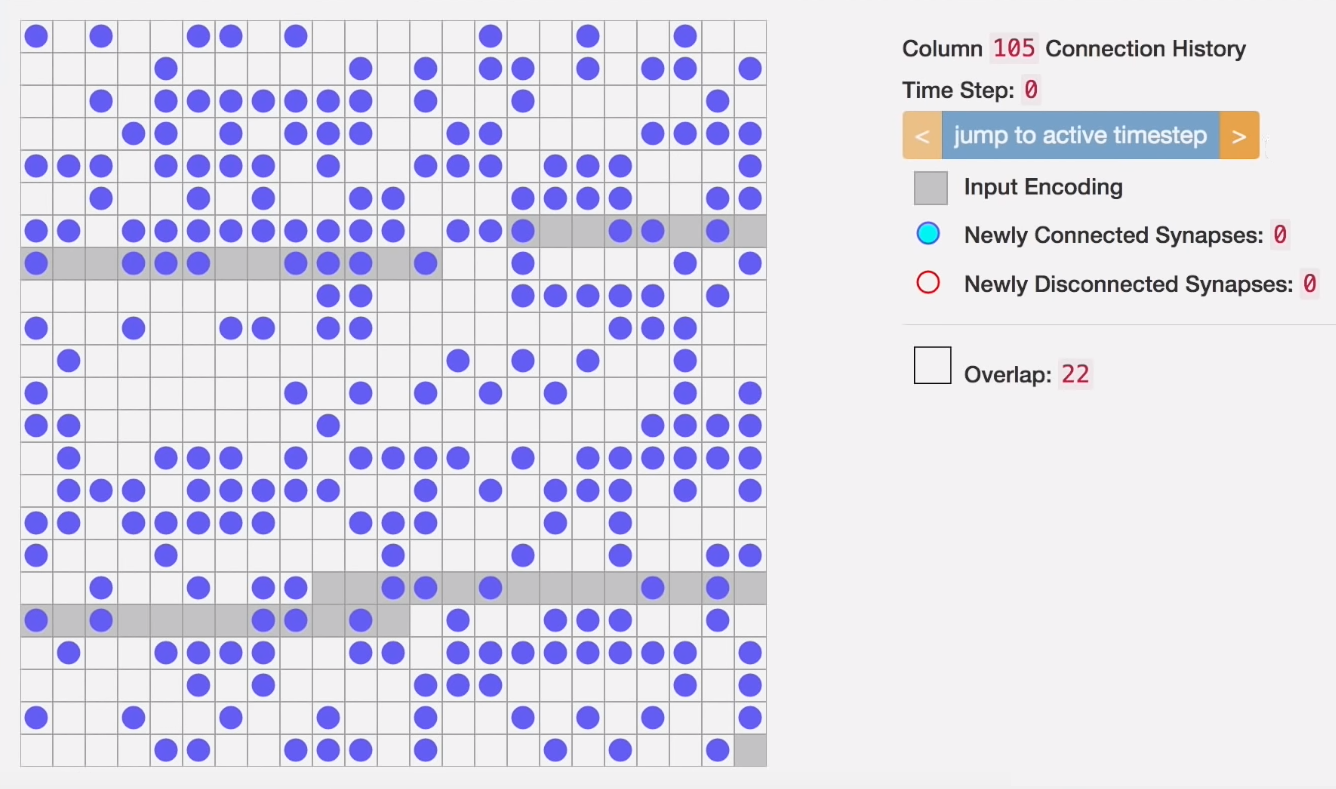
\includegraphics[width=\textwidth]{learn_ex5}
    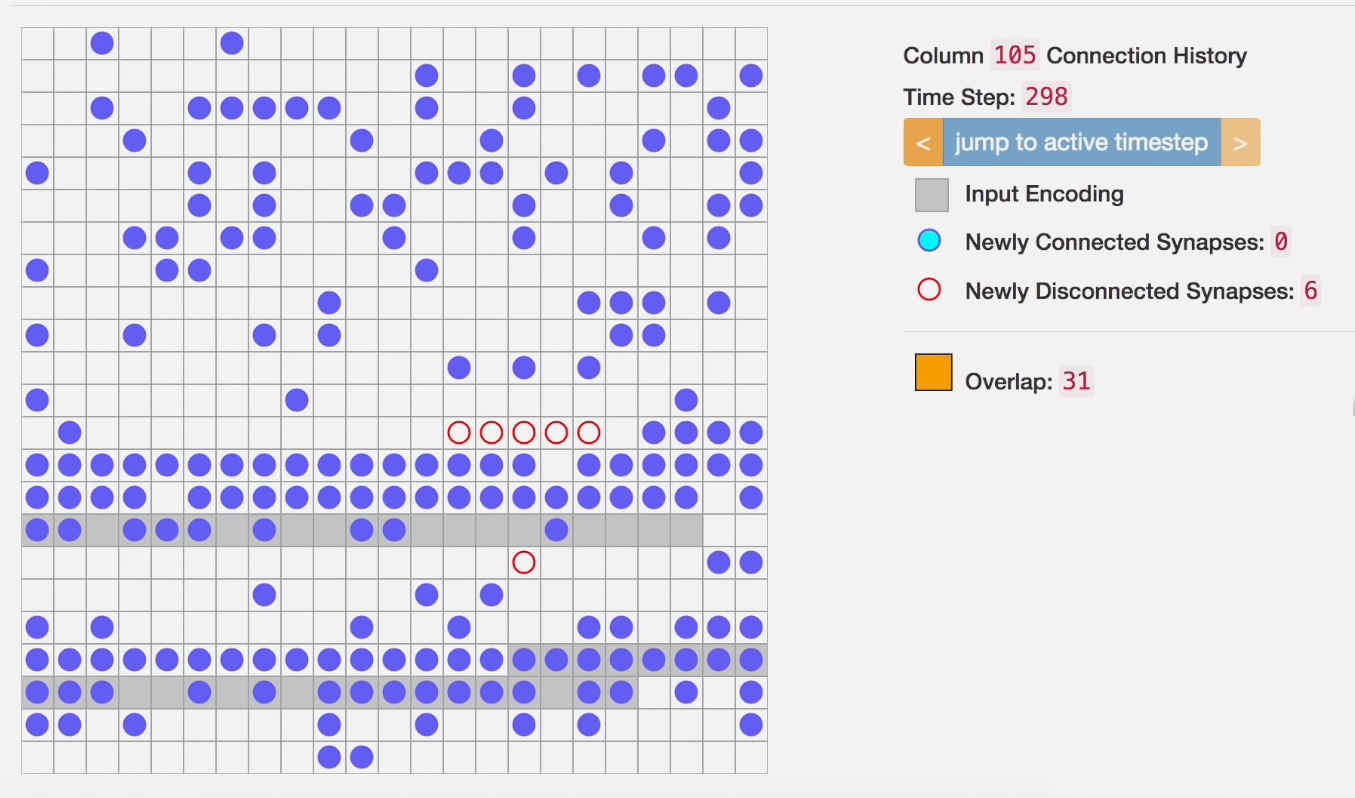
\includegraphics[width=\textwidth]{learn_ex3}
    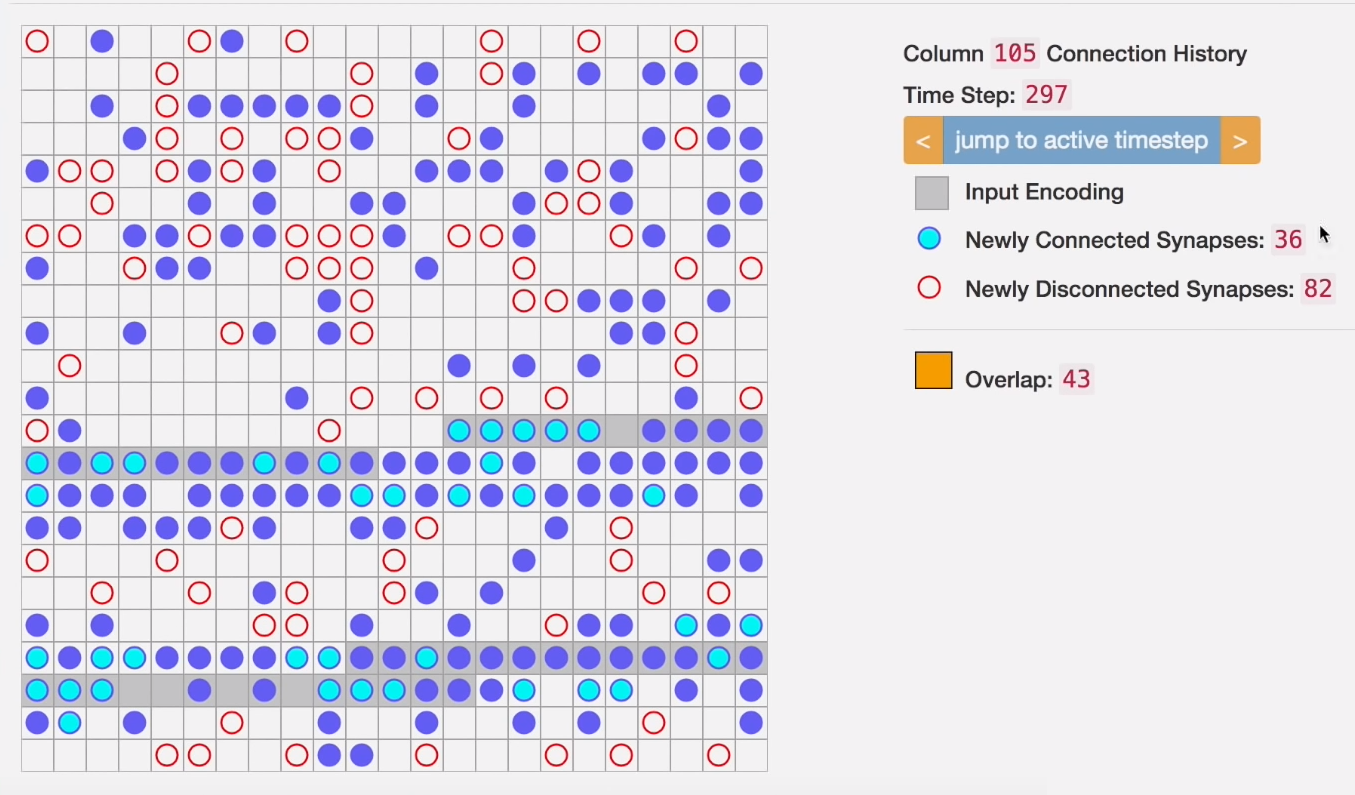
\includegraphics[width=\textwidth]{learn_ex2}
    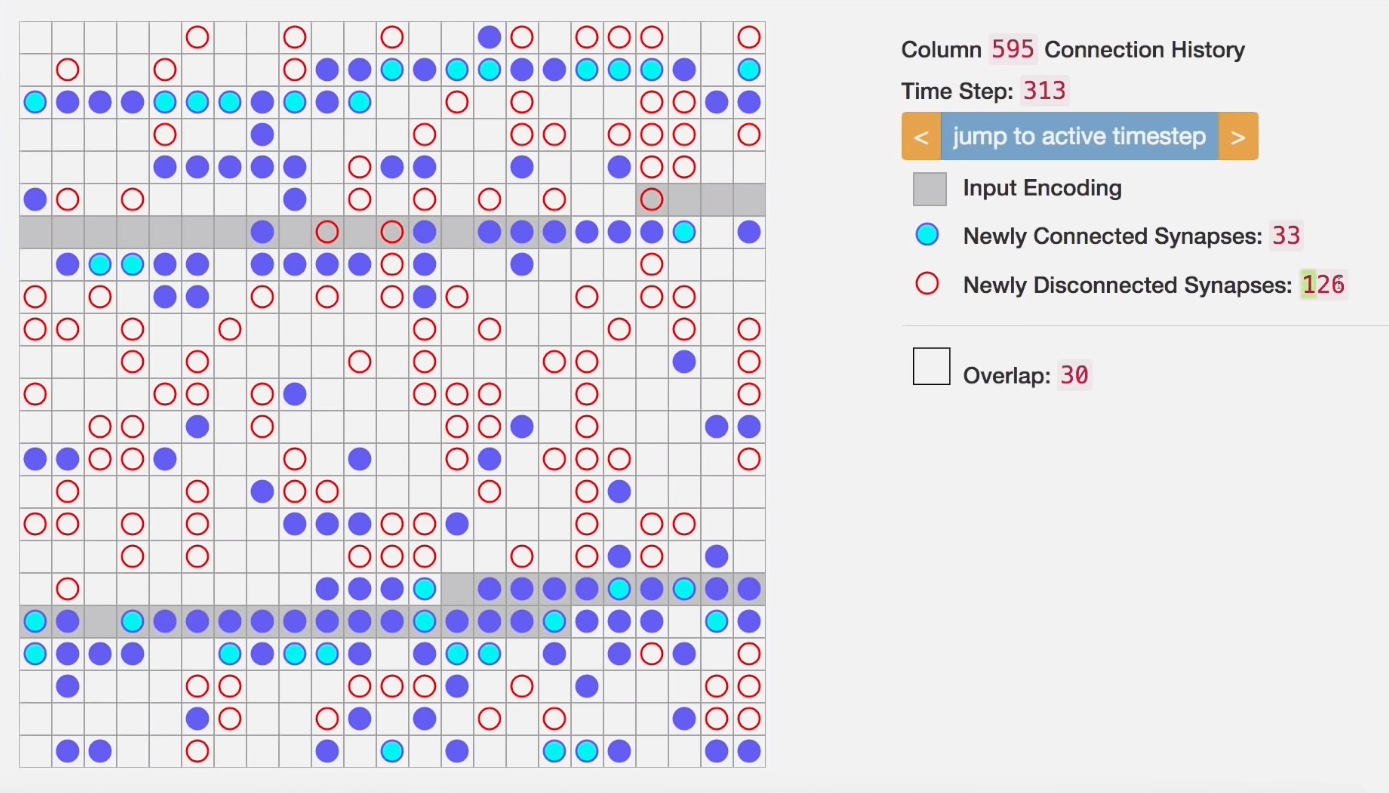
\includegraphics[width=\textwidth]{learn_ex1}
\end{frame}



% Show Pictures about granularity with vs without boosting, explain that with boosting more cells start to represent slightly different concepts


\begin{frame}[c,allowframebreaks]{Spatial Pooler - Boosting}
    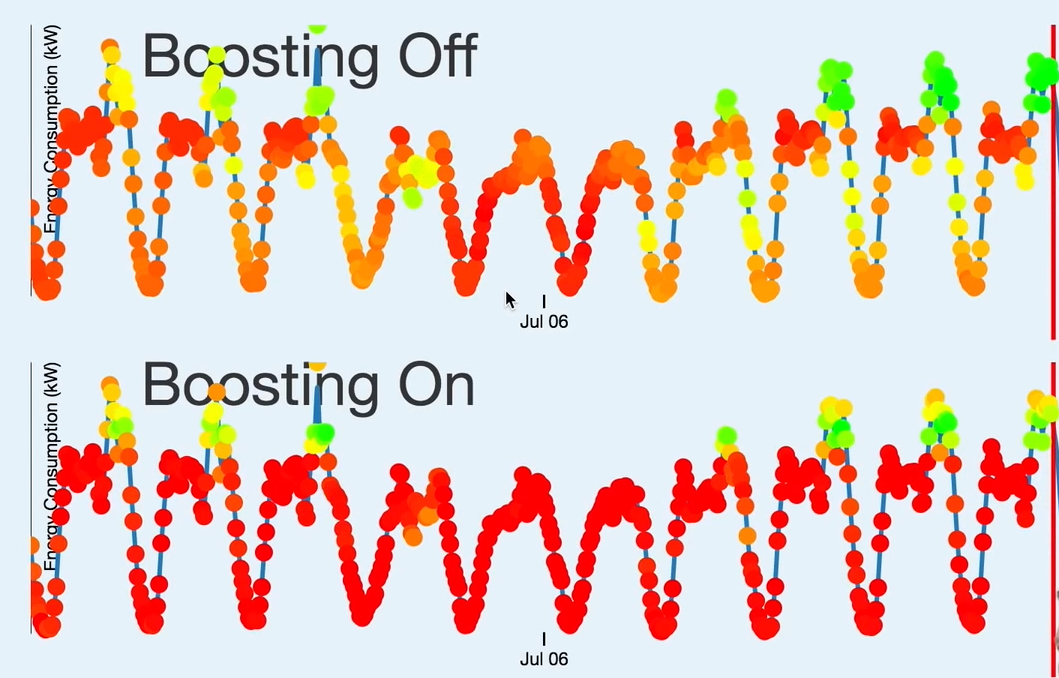
\includegraphics[width=\textwidth]{boost_ex1}
    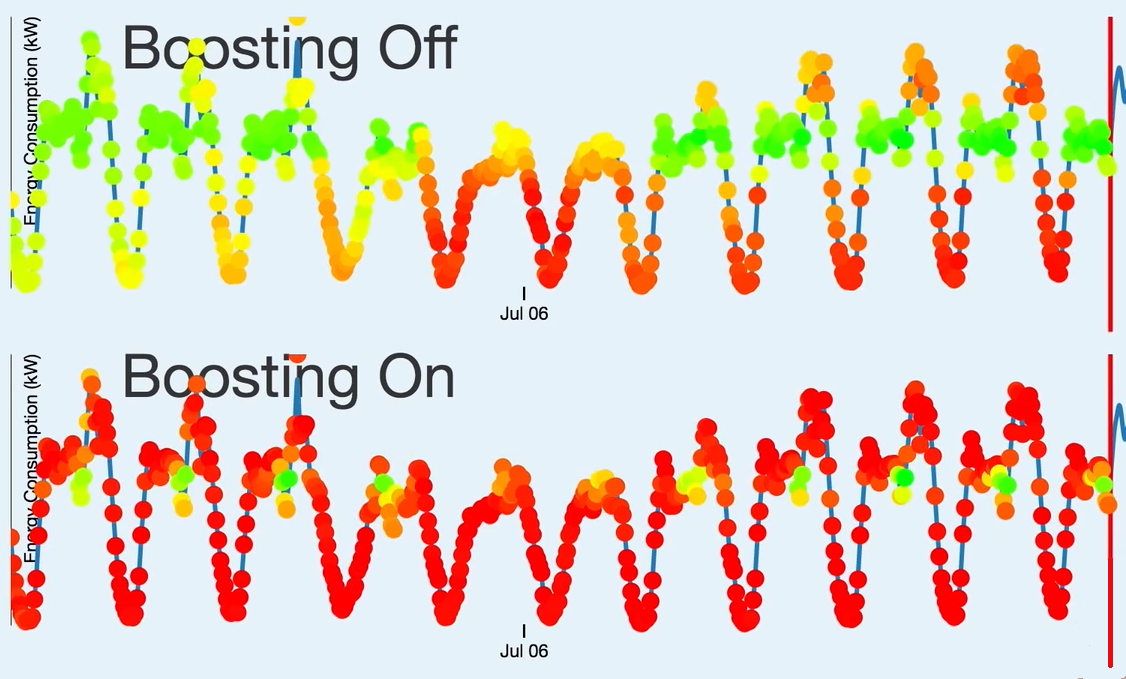
\includegraphics[width=\textwidth]{boost_ex2}
    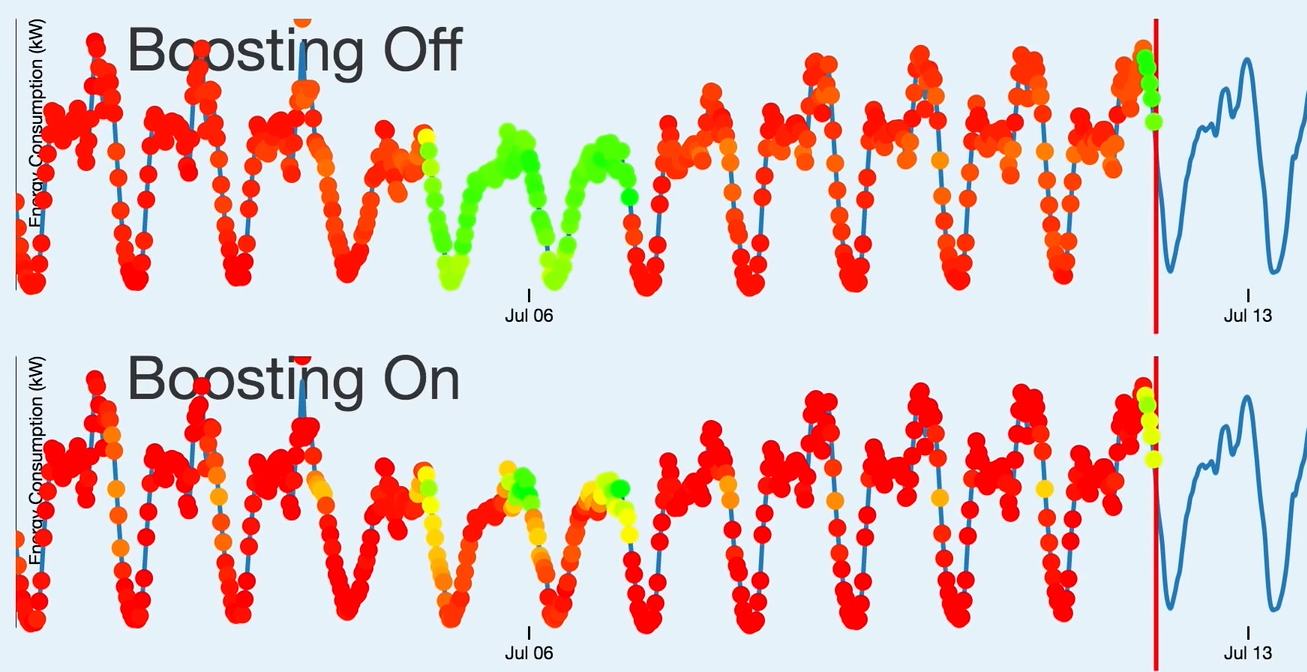
\includegraphics[width=\textwidth]{boost_ex3}
\end{frame}


\begin{frame}[c]{Spatial Pooler - Parameters}
    \Large
    \begin{itemize}[<+(1)->]
        \item Algorithm Structure (receptive field)
        \item Inhibition
        \item Learning rates
        \item Column Activity
    \end{itemize}
\end{frame}


\begin{frame}[c]{Spatial Pooler - Phases}
    \Large
    \begin{enumerate}[<+(1)->]
        \item Initializing with random variables
        \item Compute overlap scores (+Boost)
        \item Inhibition
        \item Updating Permanence values
        \item Repeat from step 2 with new input
    \end{enumerate}
\end{frame}



% SPATIAL POOLER STEPS
% 
% 1. Start with an input consisting of a fixed number of bits. These bits might
% represent sensory data or they might come from another region elsewhere in the
% HTM system.
% 
% 2. Initialize the HTM region by assigning a fixed number of columns to the
% region receiving this input. Each column has an associated dendritic segment,
% serving as the connection to the input space. Each dendrite segment has a set
% of potential synapses representing a (random) subset of the input bits. Each
% potential synapse has a permanence value. These values are randomly initialized
% around the permanence threshold. Based on their permanence values, some of the
% potential synapses will already be connected; the permanences are greater than
% than the threshold value.
% 
% 3. For any given input, determine how many connected synapses on each column
% are connected to active (ON) input bits. These are active synapses.
% 
% 4. The number of active synapses is multiplied by a “boosting” factor, which is
% dynamically determined by how often a column is active relative to its
% neighbors.
% 
% 5. A small percentage of columns within the inhibition radius with the highest
% activations (after boosting) become active, and disable the other columns
% within the radius. The inhibition radius is itself dynamically determined by
% the spread of input bits. There is now a sparse set of active columns.
% 
% 6. The region now follows the Spatial Pooling (Hebbian-style) learning rule:
% For each of the active columns, we adjust the permanence values of all the
% potential synapses. The permanence values of synapses aligned with active input
% bits are increased. The permanence values of synapses aligned with inactive
% input bits are decreased. The changes made to permanence values may change some
% synapses from being connected to unconnected, and vice-versa.
% 
% 7. For subsequent inputs, we repeat from step 3.


% \cite{cui2017htm} % <- spatial pooler




\subsection{Temporal Pooling}





\section{Implications}


% \begin{frame}[c]{Main Brain Task}
%     \pause
%     \Huge
%     What does the brain \textbf{do} \newline all the time?
% 
%     \vfill
% 
%     \pause
%     Predict. \pause Learn.
% \end{frame}
% 
% % intelligence : ability to make models
% % smart : ability to reach your goals
% % wise : picking the right goals
% 
% \begin{frame}[c]{Definition - Intelligence}
%     \Large
%     Intelligence \pause is the ability to create models. \\ \\ \pause
%     Not behaviour. Or anything else.
% \end{frame}
% 
% \begin{frame}[c]{Definition - Understanding}
%     \Large
%     Understanding \pause means to have a precise model about $<$Thing$>$.
% \end{frame}
% 
% \begin{frame}[c]{Definition - Meaning}
%     
% \end{frame}






% % \section{Conclusion}




\section{Open Questions}


\begin{frame}[c]{Open Questions}
    
\end{frame}






% 
\begin{frame}[c]{Relation to Machine Learning}
    \Large
    \pause
    Who has knowledge about Machine Learning? \newline \newline
    \pause
    How similar do you think the Brain really is?
\end{frame}




%%%%%%%%%%%%%%%%%%%%%%%%%%%%%%%%%%%%%%%%%%%%%%%%%%%%%%%%%%%%%%%%%%%%%%%%%%%%%%%%%%%%%%%%%%%%%%%%%%%



%%%%%%%%%%%%%%%%%%%%%%%%%%%%%%%%%%%%%%%%%%%%%%%%%%SOURCES%%%%%%%%%%%%%%%%%%%%%%%%%%%%%%%%%%%%%%%%%%

\section{Sources}
\begin{frame}[c,fragile,allowframebreaks]{Sources}
    \Large
    \vfill
The slides are online: \url{https://github.com/fkarg/things-to-talk-about/blob/master/htm/main.pdf} \vfill
Drop me a mail: fkarg10@gmail.com \vfill \newpage
% \bibliographystyle{plainnat}
\bibliographystyle{ieeetr}
\bibliography{references.bib}
\end{frame}


\appendix
\backupbegin

\begin{frame}[c]{Rust: Code Example}
    \begin{codeboxed}{Code Example 1}
    \inputminted[linenos, fontsize=\normalsize]{Rust}{code/code_ownership.rs}
    \end{codeboxed}
\end{frame}

\begin{frame}[c]{Rust: Code Example}
    \begin{codeboxed}{Output Nr. 1}
        \footnotesize
        \verbatiminput{code/output1.txt}
    \end{codeboxed}
\end{frame}

\begin{frame}[c]{Rust: Code Example}
    \begin{codeboxed}{Code Example 2}
    \inputminted[linenos, fontsize=\normalsize]{Rust}{code/code_ownership2.rs}
    \end{codeboxed}
\end{frame}

\begin{frame}[c]{Rust: Code Example}
    \begin{codeboxed}{Output Nr. 2}
        \footnotesize
        \verbatiminput{code/output2.txt}
    \end{codeboxed}
\end{frame}

\backupend




\end{document}


% TODO:

% Include Topics/Facts:
%
% - explain SDRs
% - explain spatial & temporal pooler
% - explain HTM
% - explain reticular activating system
% - explain gradient for Autism and that it is more 'bottom up'
% - explain 'top-down' phenomena and common biases
% - explain theory: inhibited-booost: hallucination
% - The datastructure of the brain

% Roadmap (?)
%
% - First: What is Intelligence ? (Early path, why we want to know this and why this is the most likely path)
% - Introduce the biological neuron we will be talking about (multiple dendrites, one axon, ...)
% - Introduce (SDR) Sparse Distributed Representations, in-Depth
% - Introduce the CLA
% - Introduce HTMv3 !
% - Motor movements are just very strong predictions the body 'makes happen'
%   - Flow state is where everything is exactly as predicted
% - Mistakes that happen by accidential correlation: search for good example; mistaking something to be true
% - explain gradient for Einstein/Craziness, proving vs disproving in the brain -> THC is bad
% - Mistakes that happen by top-down enforcing (e.g. the dalmatine picture, scrambled words)
% - Location-based composition: This explains mind palaces!
% - Everything is a 'conceptspace' -

% - Explain Priming based on predictive stuff (the priming-bias)
% - Explain biases based on these models
% - Explain the fact that smarter people have less Brain activity
% - Explain the bayesian-reasioning part
% - Explain how cortical columns create quite powerful models



%
